\chapter{Additional Characterization of Silicon Nanoparticles}    % First appendix chapter, i.e., Appendix A.

Here we present additional characterization of the plasma-synthesized Si nanoparticles studied in chapters 5 and 6.

\section{Transmission Electron Microscopy}
\begin{figure}
\begin{center}
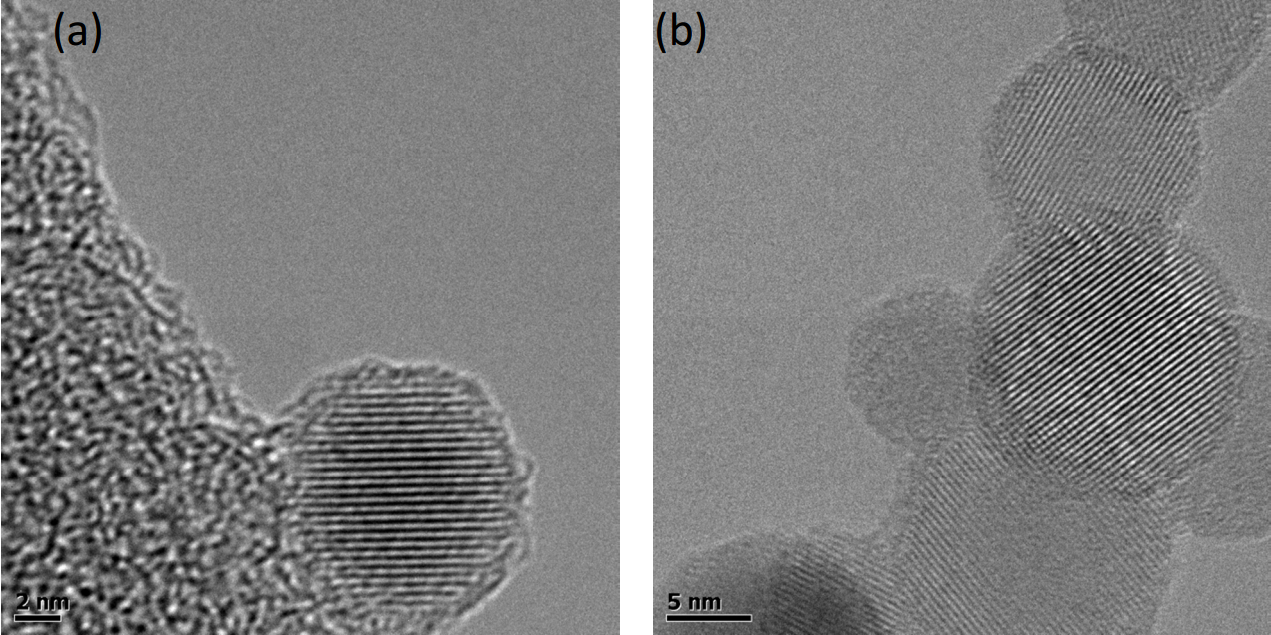
\includegraphics[width=0.75\textwidth]{./appendixC/siaddl1.png}
\caption[Transmission electron micrographs of plasma-synthesized Si NPs.]{(a) TEM image of a Si NP synthesized at a plasma power of 80 W. Fringes corresponding to the diamond Si lattice are apparent in the core of the particle, while the surface of the particle presents a disordered material. The scale bar (2 nm) is shown in the bottom left. (b) TEM image of multiple Si NPs synthesized at a plasma power of 80 W. Each particle shown presents the crystalline-core, along with the disordered-shell motif described in (a). The scale bar (5 nm) is shown in the bottom left.}
\label{f:siaddl1}
\end{center}
\end{figure}

Figure \ref{f:siaddl1} shows representative TEM images of oxygen-free silicon nanoparticles (Si NPs) studied in this work. TEM was performed by dropping a small amount of the Si NP colloid onto a thin, amorphous carbon-coated TEM grid. The displayed particles were synthesized using an RF plasma at 80W, corresponding to highly crystalline material as described in the main text. In both images displayed here, which were acquired for particles prior to attachment of surface ligands, crystalline lattice fringes are clearly visible in the Si NP core region. In addition to the crystalline core, the Si NPs displayed here lack discernible lattice fringes in proximity to the surface. Rather, each image exhibits disordered material on the surface, which we suggest is consistent with amorphous silicon material. We point out that this interpretation is also consistent with under-coordinated atoms as noted in FTIR, as well as in the asymmetry to lower frequency of the TO vibrational mode observed experimentally and theoretically in Raman (see Chapter 5 and Appendix D). In previous work by Panthani \emph{et al.}, a disordered layer around Si NPs visualized by TEM was attributed to organic ligands \cite{panthani2012graphene}. The TEM images in Panthani's work differ from those presented here in that Panthani collected Raman using a graphene substrate. The graphene substrate is atomically thin and yields minimal scattering of the electron beam. It also presents a uniform network which is readily subtracted from the image background. These factors provide a greatly elevated contrast in comparison to the amorphous carbon substrate used here. Amorphous carbon is unlikely to provide sufficient contrast for the observation of organic ligands \cite{panthani2012graphene}. We therefore suggest the disordered shell visible in Fig. \ref{f:siaddl1} is an amorphous surface layer comprising silicon. This notion is supported in the reference described above. In addition to alkyl-passiavted Si NPs, Panthani and co-workers also examined hydrogen-passivated Si NPs and observed a disordered surface layer despite the absence of alkyl ligands, consistent with our suggestion of an amorphous silicon surface layer \cite{panthani2012graphene}.

\section{Fourier Transform Infrared Spectroscopy}
Figure \ref{f:siaddl2} displays an FTIR spectrum for a Si NP ensemble synthesized at a plasma power of 80W. The intense peaks at 2140 cm$^{-1}$, 2110 cm$^{-1}$, and 2080 cm$^{-1}$ are assigned to stretching modes in SiH$_3$, SiH$_2$, and SiH, respectively. Considering the tetrahedral coordination environment of the diamond crystal structure, the presence of silicon atoms coordinated to more than one hydrogen is strongly suggestive of dangling silicon bonds inconsistent with a crystalline, ordered network. Along with photoluminescence spectroscopy data suggesting the persistence of amorphous material even for "crystalline" samples synthesized at high plasma powers, the data in Figures \ref{f:siaddl1} and \ref{f:siaddl2} lead us to hypothesize that Si NPs possess a disordered surface constituting an amorphous silicon shell. 

\begin{figure}
\begin{center}
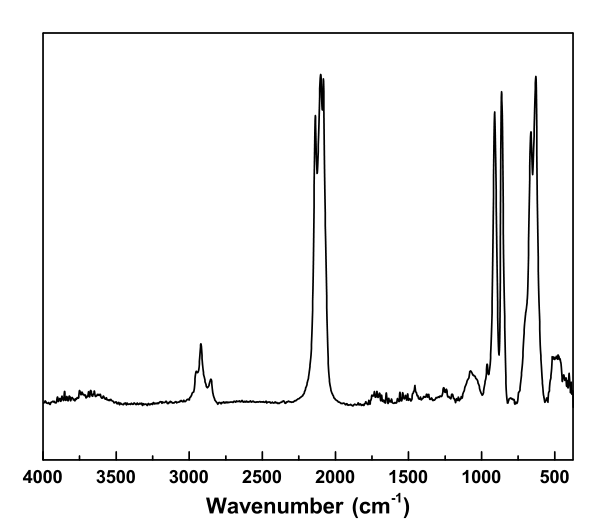
\includegraphics[width=0.5\textwidth]{./appendixC/siaddl2.png}
\caption[FTIR absorbance spectrum of plasma-synthesized, crystalline Si NPs.]{FTIR absorbance spectrum of crystalline Si NPs synthesized at a plasma power of 80 W. Si-H stretching modes are evident as the cluster of peaks near $\sim$2100 cm$^{-1}$, with the peaks at 2140 cm$^{-1}$, 2110 cm$^{-1}$, and 2080 cm$^{-1}$ corresponding to SiH$_3$, SiH$_2$, and
SiH, respectively.}
\label{f:siaddl2}
\end{center}
\end{figure}

\section{Time-Resolved Photoluminescence Over a Longer Time Window}
Figure \ref{f:siaddl3} displays the high-energy PL decay dynamics of 2.6 nm-diameter crystalline Si NPs over a time window spanning 0 - 800 ps. The data are fit to a bi-exponential decay function, yielding time constants of 20 and 151 ps, respectively. The time constants $\tau_2$ reported in Table \ref{table:amsiT1} of the manuscript are derived from fitting PL decay data over the 0 - 800 ps time window. The reported time constants $\tau_1$ are derived from the fits displayed in the manuscript, which measure a shorter time window (0 - 120 ps) and are better suited for the resolution of faster decays. This is due to the streak camera used for the detection of PL. Streak cameras inherently yield decreasing temporal resolution with increasing observation windows.

\begin{figure}
\begin{center}
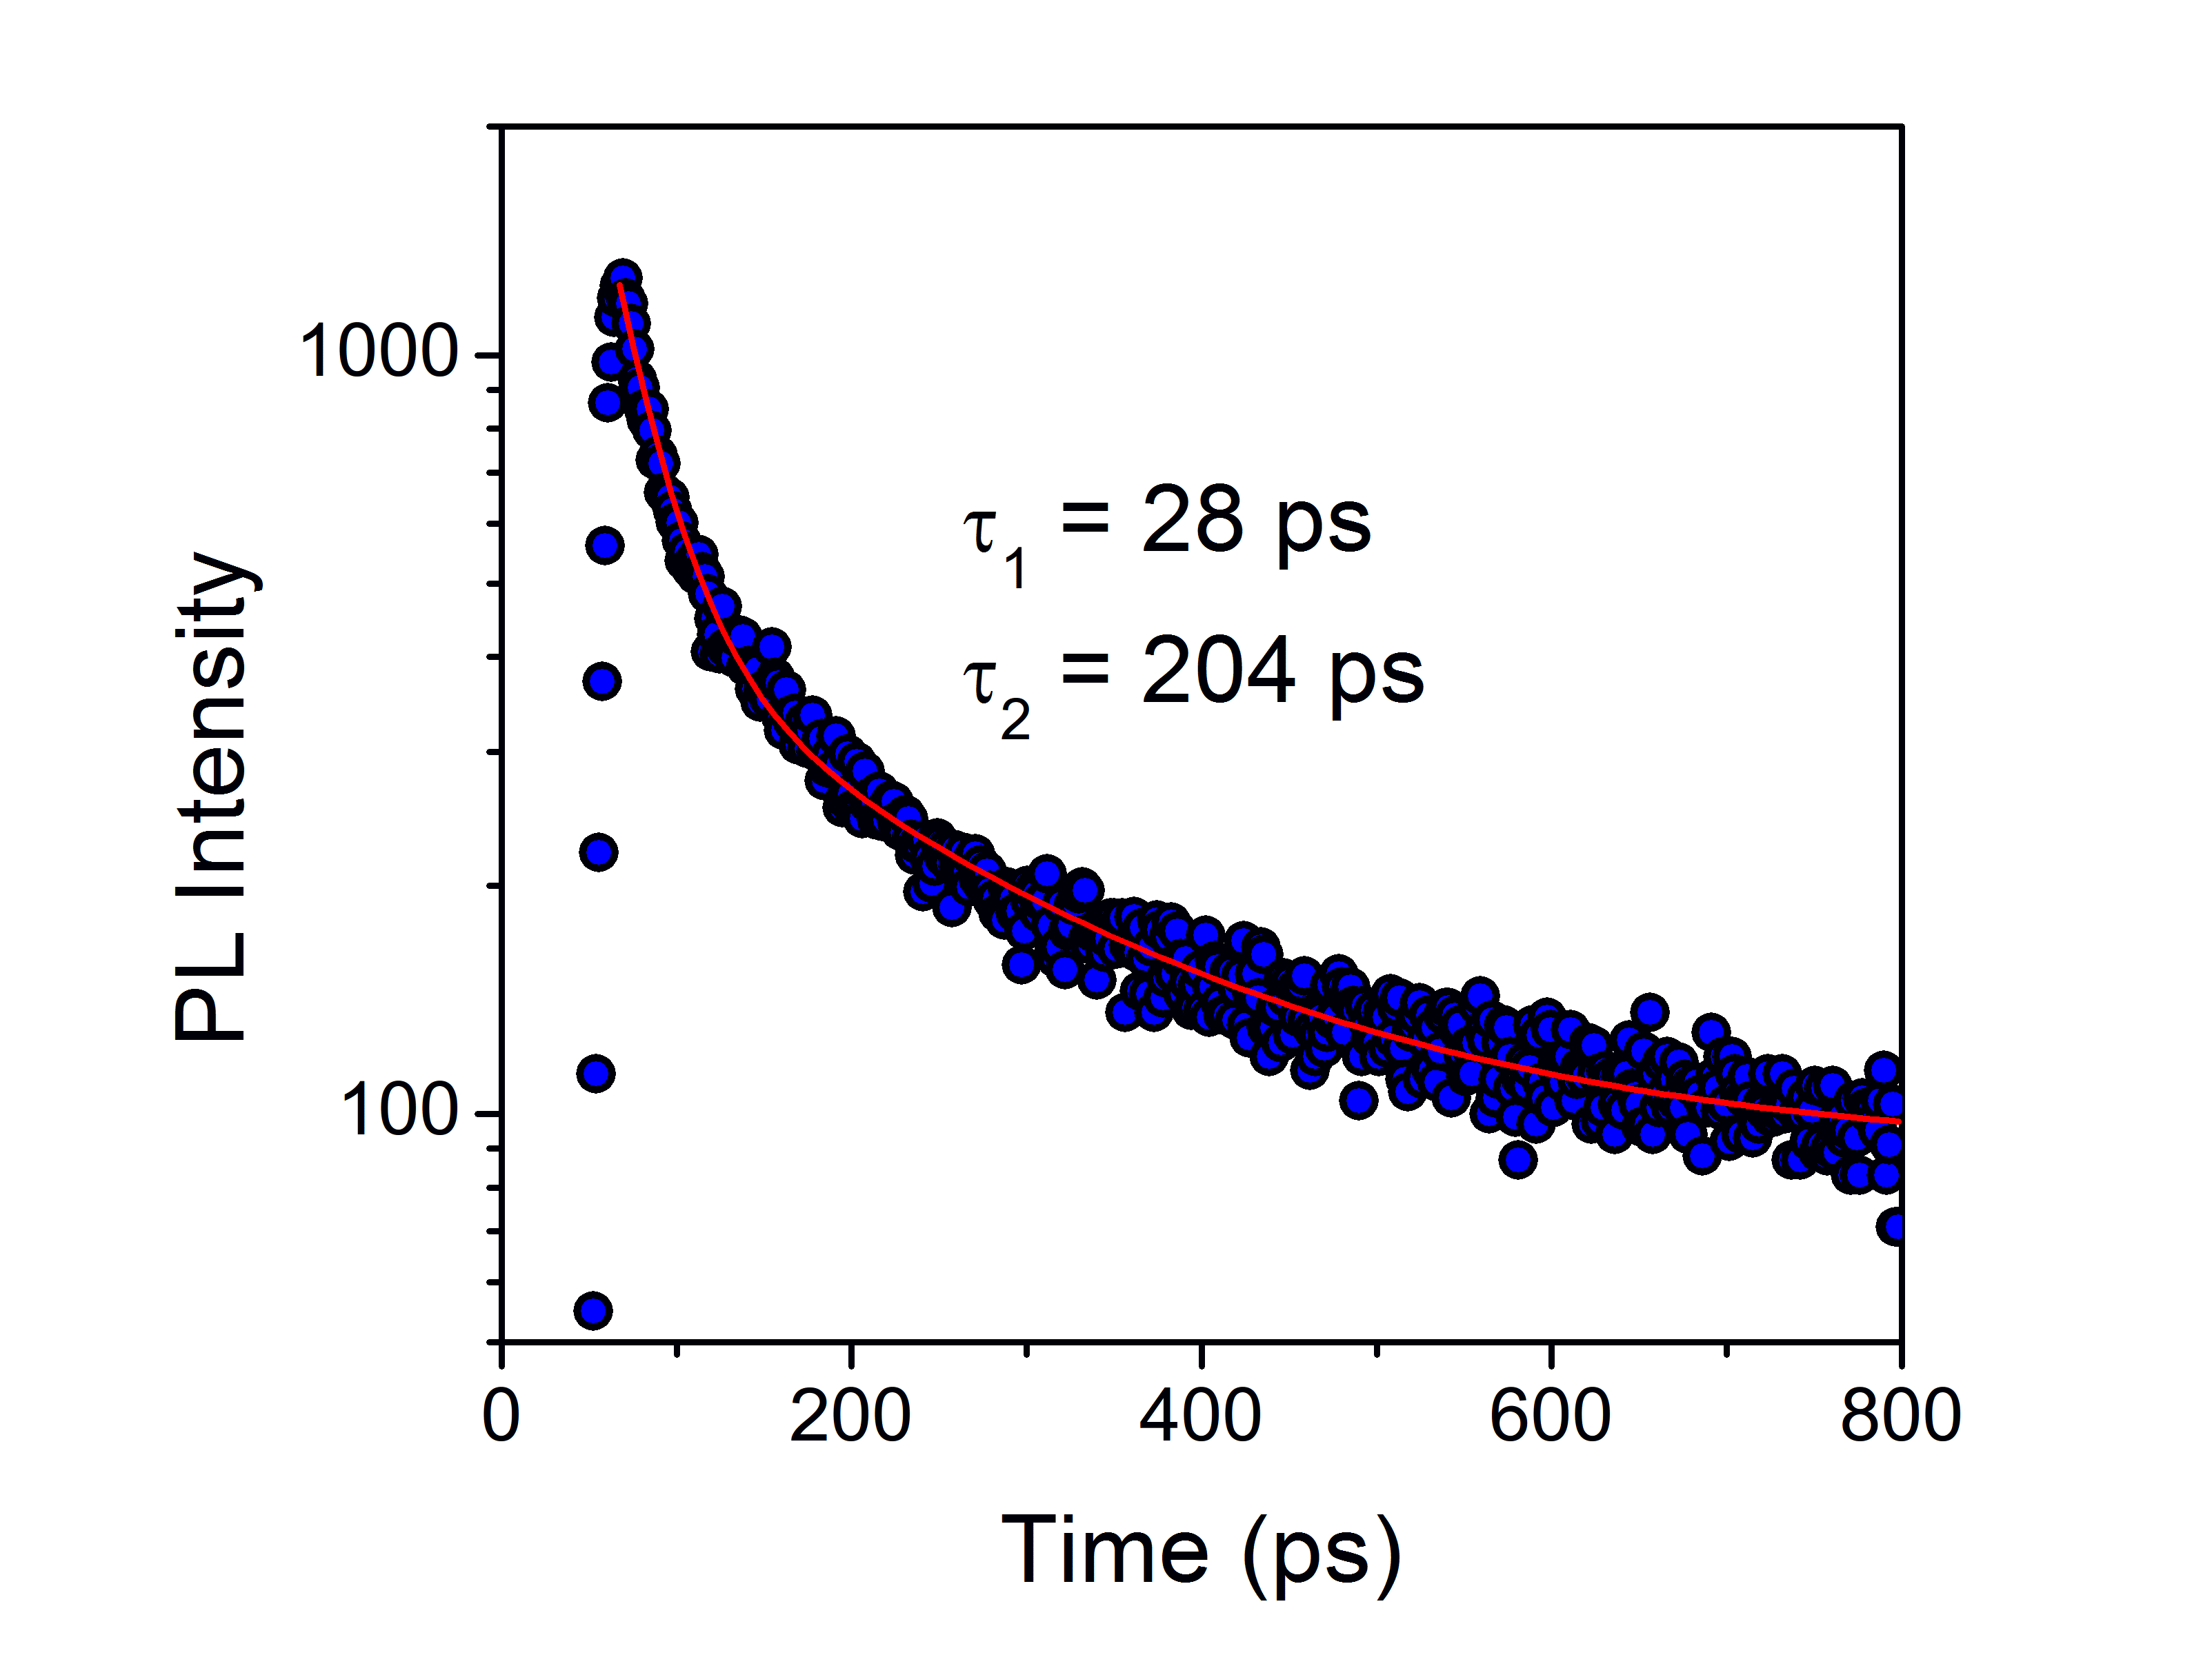
\includegraphics[width=0.7\textwidth]{./appendixC/siaddl3.png}
\caption[Picosecond PL dynamics over the 0 - 800 ps.]{Time-resolved PL dynamics spectrally integrated from 475 nm to 525 nm. The solid red line indicates a fit of the data to a bi-exponential decay function. Time constants obtained from fitting are displayed on the figure.}
\label{f:siaddl3}
\end{center}
\end{figure}

\section{Examining the Relative Quantities of Amorphous and Crystalline Material}
To estimate relative quantities of crystalline and amorphous Si present in each sample, we utilize a fitting procedure outlined in work by Smit and Van Swaaij \cite{smit2003determining}. First, the Raman spectrum of amorphous Si was recorded. We utilized CVD-grown amorphous Si. The Raman spectrum of amorphous Si was fitted to the sum of four Lorentzian lineshapes, representing the LA, TA, LO, and TO phonon modes. A fitted Raman spectrum with each of these modes indicated is shown in Figure \ref{f:siaddl4}. This Raman spectrum was then scaled to match the intensity of a Si NP Raman spectrum at the LA phonon peak center (300 cm$^{-1}$). This mode was chosen because nanocrystalline Si does not have a peak in this spectral region; any intensity in this region is therefore a contribution from amorphous Si. After scaling, the amorphous Si Raman spectrum was subtracted from the Si NP Raman spectrum, leaving only the crystalline contribution. The TO phonon peak areas of the crystalline contribution and amorphous Si were then used to calculate the fraction of amorphous material, $\gamma$, as shown below in Equation \ref{eq:siaddl1}:
\begin{equation}\label{eq:siaddl1}
\gamma = \frac{A_{TO}^{c}}{A_{TO}^{c} + 0.8 \cdot c \cdot A_{TO}^{a}}
\end{equation}
In Eq. \ref{eq:siaddl1}, $A_{TO}^{c\left(a\right)}$ is the crystalline (amorphous) TO phonon peak area. The crystalline contribution is obtained as described above from the Si NP Raman spectra. The amorphous TO phonon peak area is obtained by fitting the amorphous Si Raman spectrum as described above. $C$ is the scaling constant needed to normalize the amorphous Si spectrum to the Si NP Raman spectrum at the LO phonon peak center. Finally, the factor of 0.8 accounts for differences in the Raman cross-section for the TO phonon mode between crystalline and amorphous Si \cite{smit2003determining}.

\begin{figure}
\begin{center}
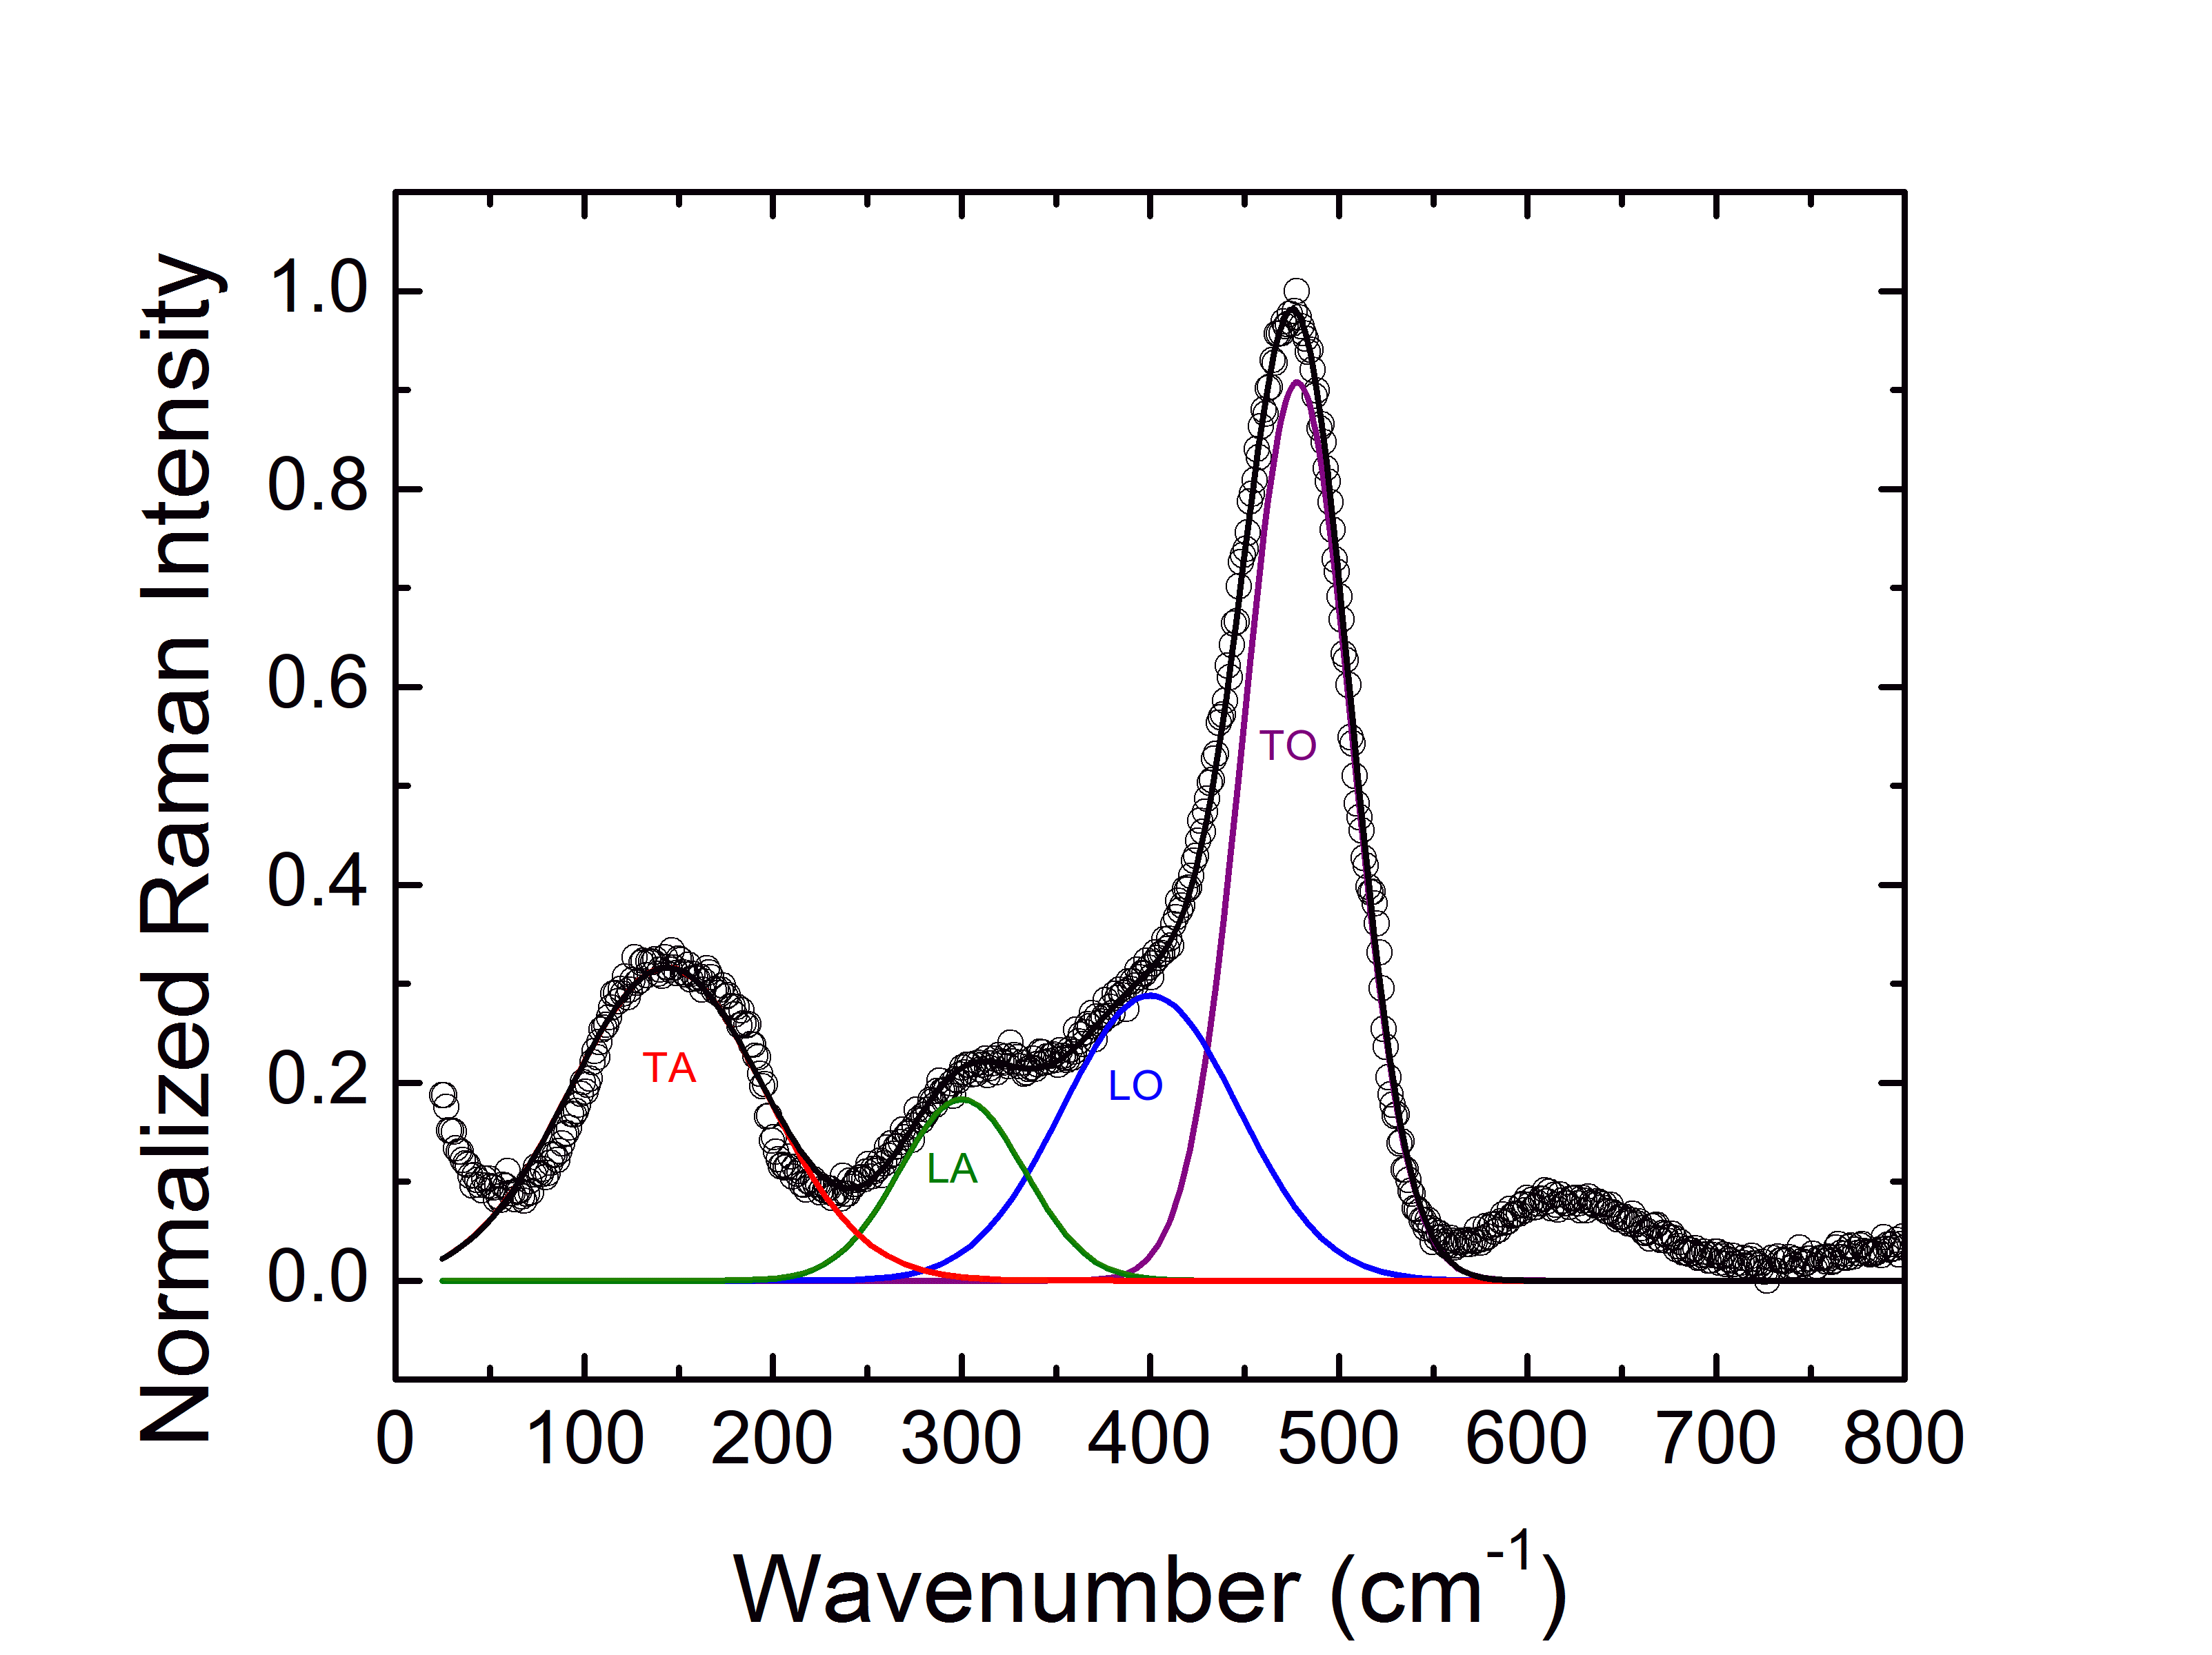
\includegraphics[width=0.7\textwidth]{./appendixC/siaddl4.png}
\caption[Raman scattering spectrum of CVD-grown amorphous Si.]{Raman scattering spectrum of CVD-grown amorphous Si (circles). The spectrum was fit the sum of four Lorentzian lineshapes, which are indicated by the solid lines in the figure. The phonon mode corresponding to each peak is also labeled (TO = Transverse optical, LO = longitudinal optical, LA = longitudinal acoustic, TA = transverse acoustic).}
\label{f:siaddl4}
\end{center}
\end{figure}
 
